\chapter{Fundamentação Teórica}
\label{cap:fundamentacao_teorica}

As cadeiras de rodas motorizadas proporcionam conforto, segurança, rapidez e prevenção de lesões nos membros superiores devido ao uso repetitivo em cadeiras de rodas manuais. Contudo para a aquisição de uma cadeira de rodas motorizada exija-se um elevado capital inicial de investimento. Em uma análise do impacto orçamentário realizada pelo Departamento de Economia da Saúde, Investimento e Desenvolvimento - Ministério da Saúde-DESID/SE/MS, o preço sugerido para uma cadeira de rodas motorizada é de R\$ 4.999,00, além do custo de manutenção \cite{relatorio_sus}.

Em caso de necessidade, estas cadeiras não podem ser usadas como cadeiras de rodas manuais, pois possuem rodas pequenas para aproveitar melhor a potência dos motores e sistema de transmissão. Outro detalhe importante é que cadeiras de rodas motorizadas são geralmente pesadas e não possuem as facilidades de transportes das cadeiras manuais.

Neste capítulo é apresentada toda a fundamentação teórica utilizada para a criação do produto desenvolvido. Dividido em seções, o capítulo aborda os princípios do \textit{Power Train} (Alimentação e Motores) e Controle Eletrônico utilizados.

Na seção \textit{Power Train} são apresentados conceitos relacionados a motores e baterias, já na seção Controle são apresentados controladores analógicos de motores (ponte H), interface de controle do usuário, microcontroladores, arquitetura, linguagens de programação, testes de \textit{software} e tecnologias.

\begin{comment}
Quando a parte de estrutura estiver na fundamentação teórica, trocar os dois últimos parágrafos dessa introdução por:

-----------------------------
Neste capítulo é apresentado
	\item \textit{Power Train} (Alimentação e Motores)
	\item Estrutura Mecânica
	\item Controle Eletrônico
\end{itemize}

Na seção \textit{Power Train} são apresentados conceitos relacionados a motores e baterias. Em \textit{Estrutura Mecânica} são apresentadas as ferramentas computacionais utilizadas, conceitos a cerca de materiais e cálculos estruturais. Na seção \textit{Controle} são apresentados controladores analógicos de motores (ponte H), interface de controle do usuário, microcontroladores, arquitetura, linguagens de programação, testes de \textit{software} e tecnologias.
-----------------------------
\end{comment}

\section{Estrutura}

	\textbf{Liga Metálica}


	Com o objetivo de confeccionar a estrutura que suportará os motores e baterias, é necessário observar alguns conceitos dos materiais que são relevantes ao projeto, bem como o custo, já que este trabalho se trata de um trabalho universitário.

	De acordo com a matéria publicada por Infomet, a dureza e resistência da liga deve-se ao enriquecimento superficial nos aços que é suportada por um núcleo tenaz. Sabe-se que vários tipos de aço apresentam boas condições para essa finalidade. Para tanto, deve-se levar em consideração que a cementação exige tratamento térmico relativamente complexo, o que faz com que a escolha do aço não pode ser feita baseada somente na aplicação final do material, mas também levando em conta as condições térmicas que o material irá sofrer \cite{ensaio_fadiga}. Para esse trabalho, o material estará exposto a condições de temperatura ambiente, o que não será uma variável preocupante. Dessa forma, os esforços mecânicos serão os que merecem devida atenção.

	Levando em consideração principal o aspecto financeiro verificou-se dois tipos de ligas que podem ser utilizadas nesse trabalho: SAE 1020 e SAE 1040. De acordo com a fornecedora de aço Favorit, o aço SAE 1040 apresenta boa resistência mecânica, boa usinabilidade e baixa soldabilidade. Estes aços não apresentam as mesmas características mecânicas e metalúrgicas apresentadas pelos aços especiais, pois em seus processos de fabricação não são controlados o tamanho de grão austenítico, os níveis de gases dissolvidos, o grau de pureza, etc. As faixas de composições químicas dos aços comerciais são apenas orientadas pela norma NBR 6006 ou pelas normas internacionais tipo SAE, AISI, ou DIN, portanto, não há garantias de que os teores dos elementos químicos principais ou residuais estejam estritamente dentro dos limites especificados por estas normas. Além disto, nos aços comerciais, não são garantidas as faixas de temperabilidade conforme as normas NBR ou SAE \cite{favorit}. Como outra opção, o aço SAE 1020 é um dos aços ao carbono mais utilizado como aço para cementação com excelente relação custo benefício quando comparado com aço para o mesmo propósito \cite{metals}.

	De acordo com um experimento realizado no trabalho de conclusão de curso do Fernando Ickert, através da análise visual das amostras foi possível observar que os materiais que possuem maior ductilidade (aço SAE 1020 e aço SAE 1045), apresentaram escoamento com maior facilidade em relação aos materiais menos dúcteis (aço inoxidável AISI 304). A partir disto, foi possível verificar com maior clareza a propagação da trinca devido à compressão e tração do corpo de prova, ao longo do ensaio até sua ruptura por fadiga, pois as amostras de aço SAE 1020 e aço SAE 1045 apresentaram uma considerável deformação antes de atingir a ruptura, ao contrário do que aconteceu com um material dúctil-frágil no caso do aço inoxidável AISI 304, que não apresentou uma variação visível em sua deformação e acabou rompendo de maneira inesperada \cite{ensaio_fadiga}.

	Conforme a fornecedora de aço Açosport, Características e propriedades mecânicas dos aços SAE 1020, os aços SAE 1020 são aços carbonos de ligas metálicas constituídas basicamente de ferro, carbono, silício e manganês, apresentando também outros elementos inerentes ao processo de fabricação, em percentuais controlados. O aço carbono SAE 1020 é um dos aços mais utilizados, devido a sua baixa temperabilidade, excelente forjabilidade e soldabilidade, porém sua usinagem é relativamente pobre. Esse aço é indicado para parafusos, trefilados duros, chassis, discos de roda, peças em geral para máquinas, tubos soldados e veículos submetidos a esforços pequenos e médios. Este tipo de aço é altamente tenaz, particularmente indicado para fabricação de peças que devam receber tratamento superficial para aumento de dureza, principalmente cementação. O aço SAE 1020 é utilizado ainda para eixos em geral, forjados \cite{acosport}.

	Por conta da facilidade de compra do SAE 1020 e especificações mecânicas descritas acima, o grupo optou por esse material para a realização da estrutura do dispositivo de locomoção automatizada. O material atende todas as especificações mecânicas para aguentar as cargas exigidas.

	\textbf{Resistência a Rolagem}

	Segundo \cite{propulsao_cadeira}, os fatores que determinam a resistência ao rolamento são: os coeficientes de atrito das rodas traseiras e dianteiras, o peso total do sistema (cadeira e usuário), a superfície em que a cadeira está sendo impulsionada e a distribuição de peso entre as rodas traseiras e dianteiras através do centro de massa (Cm).

	A figura \ref{fig:diagrama_variaveis} é um diagrama que ilustra as variáveis que determinam a resistência de rolagem da cadeira de rodas manual. Estas variáveis são: o comprimento da roda (\textit{dwb}), a distância horizontal do eixo das rodas traseiras ao centro de massa (\textit{x}) e a distância horizontal do eixo das rodas dianteiras ao centro de massa (\textit{dwb-x}).

	As forças presentes no diagrama representam as forças peso das rodas traseiras (\textit{fr}) e das dianteiras (\textit{fc}), que fazem parte das forças de resistência ao rolamento: \textit{fr,rr} das rodas traseiras e \textit{fc,rr} das rodas dianteiras. Nas equações abaixo: $\mu$ é o coeficiente de fricção de rolagem, $m$ é a massa e $g$ é a aceleração da gravidade \cite{propulsao_cadeira}.

	\begin{equation}
		f_r=m*g\frac{(dwb-x)}{dwb} ; f_{r,rr}=\mu*f_r
	\end{equation}
	\begin{equation}
		f_c=m*g\frac{x}{dwb} ; f_{c,rr}=\mu*f_c
	\end{equation}
	\begin{equation}
	f_rr=f_{c,rr}+ f_{r,rr}
	\end{equation}

	A resistência ao rolamento $frr$ é, por fim, a soma das resistências das rodas dianteiras e traseiras.

	\begin{figure}[!h]
		\centering
		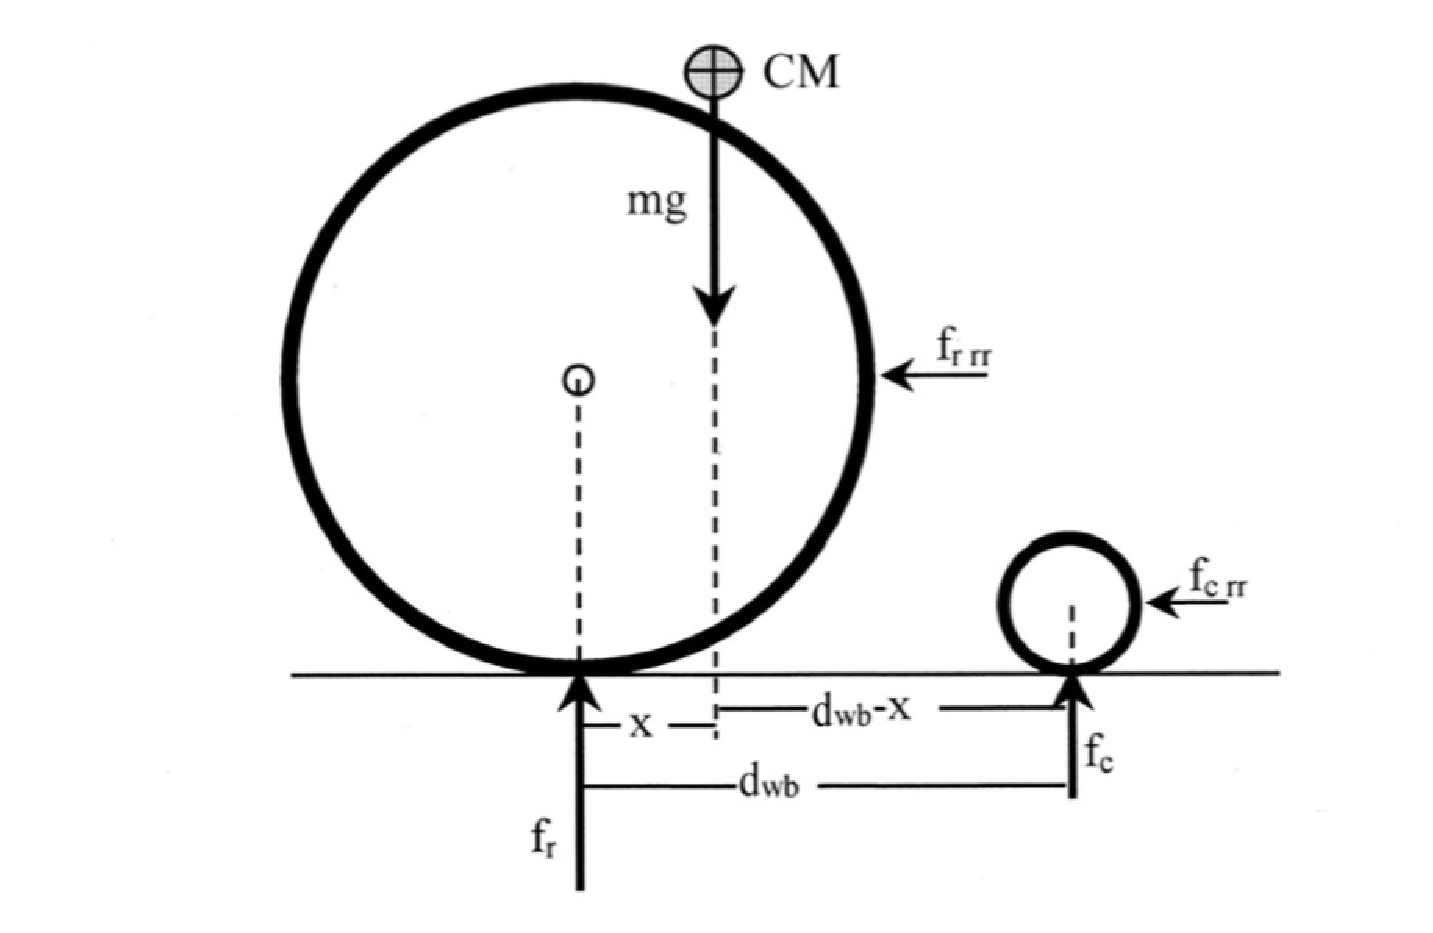
\includegraphics[width = 0.7\textwidth]{figuras/resultados/diagrama_variaveis}
		\caption{Diagrama das variáveis que determinam a resistência de rolagem da cadeira de rodas manual. \cite{propulsao_cadeira}.}
		\label{fig:diagrama_variaveis}
	\end{figure}


\section{\textit{Power Train}}

Para que a cadeira de rodas se movimente sem o uso de força humana, é preciso de um sistema elétrico capaz de substituir essa ação. Tal sistema deve ser composto por motores que darão o torque e a força necessária para as rodas da cadeira, e por uma fonte de energia que alimente estes motores, garantindo autonomia eficiente ao sistema, uma bateria, por exemplo.

\subsection{Motor Elétrico}

O motor elétrico é uma máquina que tem a capacidade de transformar energia elétrica em energia mecânica \cite{projeto_cadeira_rodas_inteligente}. Existem dois tipos de motores: motor de corrente alternada (CA) e os de corrente contínua (CC).

As cadeiras de rodas automáticas utilizam-se de baterias como fonte de alimentação para os motores, portanto deve-se utilizar motores de corrente contínua. Este tipo de motor é muito utilizado em projetos que necessitam de velocidades variáveis, eles também apresentam uma região de torque e potência constante e são simples de realizar a aceleração e a desaceleração \cite{manual_bateria_unipower}.

É necessário que as relações de velocidades entre os motores tenham um sistema de controle rígido de forma que o usuário consiga controlar a cadeira adequadamente. Os motores devem responder aos comandos sem que hajam erros por uma questão de segurança. Uma metodologia para o dimensionamento de sistemas de tração para veículos elétricos é baseada na dinâmica veicular e considerando três condições de operação:

\begin{itemize}
	\item Aceleração inicial
	\item Velocidade nominal
	\item Velocidade máxima
\end{itemize}

Um sistema que supre essas três condições funcionará adequadamente nos demais regimes de operação. Os parâmetros que definem essas restrições são:

\begin{itemize}
	\item Velocidade nominal do veículo
    \item Tempo especificado para o veículo atingir a velocidade nominal
    \item Velocidade máxima
    \item Massa do veículo
\end{itemize}

\subsubsection{Motor de Corrente Contínua}

O objetivo é atender as restrições de projeto com o menor requerimento de potência, ou seja, obter um perfil de torque-velocidade ótimo para o sistema de tração elétrica. Os motores de corrente contínua utilizam-se das forças eletromagnéticas para transformar energia elétrica em mecânica, eles funcionam com uma fonte retificada, ou seja, que possuem polaridade fixa.

Este tipo de motor possui dois terminais, um positivo e outro negativo que de acordo com a polaridade e o sentido da corrente controlam a repulsão dos eletroímãs e consequentemente o sentido da rotação do motor. Desta maneira, este tipo de motor seria capaz mover as rodas tanto para frente quanto para trás, promovendo mobilidade à cadeira de rodas do usuário.

Uma das maiores vantagens dos motores de corrente contínua é o controle da velocidade que é feito por drenagem de corrente para o motor. Porém são mais difíceis de serem construídos e mais propícios a problemas, gerando uma maior manutenção.

Outro problema encontrado é a alta velocidade angular. Motores de corrente contínua encontrados no mercado possuem velocidades angulares nominais entre 2500 e 2800 rpm, o que lhes confere um baixo torque. Cadeiras de rodas precisam de motores que transmitam um alto torque para movimentar suas rodas, assim, se faz necessário um sistema redutor acoplado ao eixo do motor para reduzir a velocidade angular e aumentar o torque.

\subsection{Redutor}

O redutor tem a finalidade de modificar algumas características de ventiladores, bombas e motores elétricos para o acoplamento com outros dispositivos em seus eixos. Desta forma, o uso do redutor irá variar a velocidade, rotação ou torque \cite{apresentacao_andrade}.

Para que haja uma redução do torque do eixo do dispositivo gerador de energia é necessário que haja a conexão deste com um conjunto de eixos com engrenagens cilíndricas dentadas ou com um parafuso.

Por meio destas engrenagens a velocidade de rotação da transmissão é reduzida, e o contato entre engrenagens de menor ou maior número de dentes possibilita a redução de torque desejada, lembrando que a quantidade de dentes depende da variação do diâmetro da engrenagem. A figura \ref{fig:motor} representa um motor acoplado a um redutor.

Existem dois tipos principais de redutores: Engrenagens cilíndricas de dentes retos e engrenagens cilíndricas de dentes helicoidais.

As primeiras distinguem-se por transmissão de força sem deslizamento nos dentes, relação de multiplicação constante e independência de carregamento. Promove segurança de funcionamento, durabilidade, resistência a sobrecargas, fácil manutenção e dimensões reduzidas em relação a potência.

As engrenagens cilíndricas de dentes helicoidais apresentam a vantagem de terem um funcionamento muito suave. Elas trabalham com relevante escorregamento de um dente sobre outro. Sua utilização permite transmissões silenciosas, sem vibrações e choques. O número de dentes mínimo poderá ser inferior ao das engrenagens cilíndricas de dentes retos, e a relação de transmissão poderá ser maior. Sendo a superfície de contato muito reduzida, se tem grandes pressões, por isso as engrenagens helicoidais são mais usadas.

\begin{figure}[!htb]
	\centering
	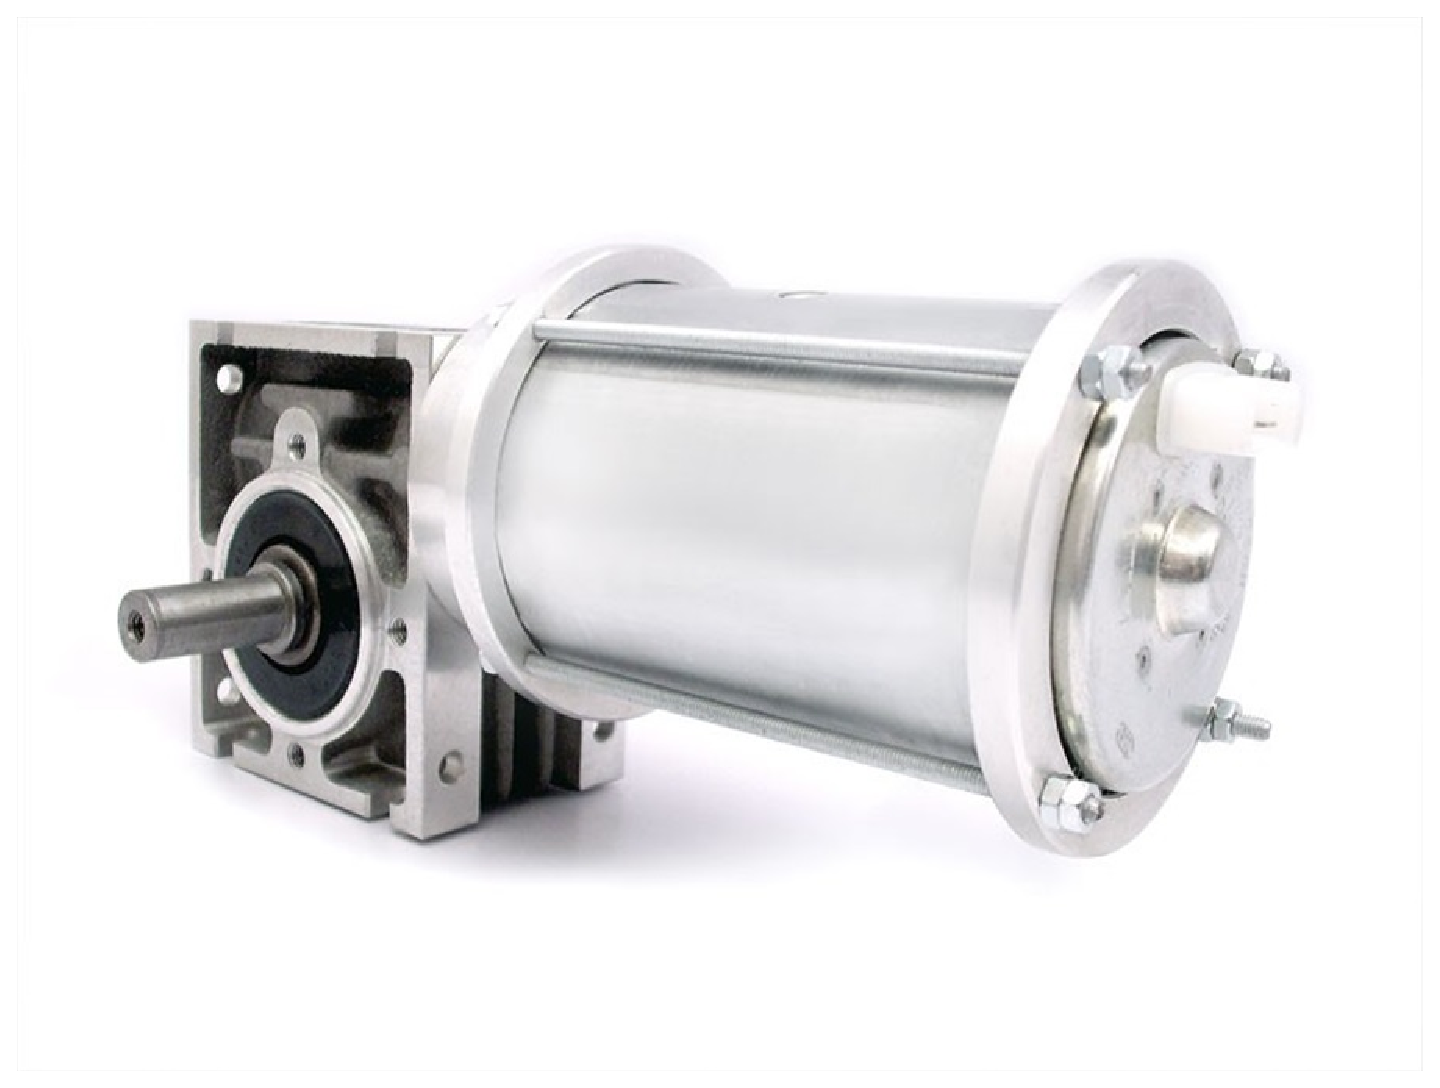
\includegraphics[keepaspectratio=true,scale=0.5]{figuras/referencialteorico/motor}
	\caption{Motor de corrente contínua acoplado a um redutor}
	\label{fig:motor}
\end{figure}

\subsection{Bateria}

Baterias são dispositivos que transformam energia química em elétrica e vice-versa. Por ser um processo reversível, as baterias podem ser carregadas e descarregadas várias vezes. Hoje no mercado existem vários tipos de baterias, com diferentes condições nominais.

A bateria adequada ao projeto seria uma bateria de chumbo ácida, muito utilizada em veículos devido a seu fácil acesso e baixo custo. Atualmente ela já é utilizada em cadeiras de rodas elétricas. Este é o tipo menos eficiente de bateria, com a pior relação peso/energia, mas em compensação é a tecnologia mais barata.

Inventadas em 1859 pelo físico francês Gaston Planté, é muito utilizada hoje em dia em diferentes áreas, como automóveis, sistemas de fornecimento de energia elétrica ininterrupta (\textit{no-breaks}) e cadeiras de rodas elétricas.

Um grande problema foi solucionado na década de 70, onde pesquisadores conseguiram desenvolver uma bateria de chumbo-ácido livre de manutenção, podendo operar em qualquer posição. Nesta bateria, o invólucro foi selado e o eletrólito líquido foi transformado em separadores umedecidos.

As baterias SLA (bateria selada chumbo-ácido), também conhecida como \textit{Gelcell}, estão livre do famoso efeito memória, em que as baterias perdem autonomia conforme a quantidade de ciclos, de carga e recarga. Além disso, deixar a bateria em carga flutuante por um longo período não causa nenhum dano.

A bateria de chumbo-ácido tem a melhor retenção de carga entre todas as baterias recarregáveis. As baterias de SLA descarregam, em média, aproximadamente 40\% da sua energia armazenada em 1 ano, já uma de NiCd se auto descarrega na mesma quantidade em 3 meses.

As baterias SLA devem sempre ser armazenadas carregadas. Deixar a bateria descarregada causa sulfação, uma condição que torna difícil, se não impossível, de se recarregar as baterias. A bateria SLA consegue fornecer entre 200 e 300 ciclos de carga/descarga.

Vantagens:

\begin{itemize}
	\item A mais barata em termos de custo por Watt hora;
	\item Segura e durável quando utilizada corretamente;
	\item Auto descarga está entre as mais baixas entre as baterias com sistema de recarga;
	\item Não exige muita manutenção e não tem o efeito memória.
\end{itemize}

Limitações:

\begin{itemize}
	\item A bateria não pode ser armazenada em completa descarga, a tensão tem de estar acima de 2,10V;
	\item Densidade baixa da energia;
	\item Ciclo de carga/descarga limitado;
	\item O eletrólito e o conteúdo da carga podem causar danos ambientais;
	\item Imprópria para dispositivos de mão que exigem tamanho compacto.
\end{itemize}

\subsubsection{Carregando baterias}

O tempo de carga de uma bateria de Chumbo-Ácido (selada) é de 12 a 16 horas. Com correntes de carga maiores, e métodos de carga multi-estágios, o tempo de carga pode ser reduzido para 10 horas ou menos. Durante a carga em corrente constante, a bateria carrega 70\% em aproximadamente 5 horas, os 30\% restantes são completados por uma lenta carga de pico. A corrente de pico dura outras 5 horas e é essencial para o bem estar da bateria.

\section{Controle}

Desde a primeira patente de cadeira de rodas elétrica em 1937 \cite{patent_cadeira_rodas_eletrica}, diversos modelos de cadeiras de rodas motorizadas foram desenvolvidos. As mais diversas interfaces humano-computador foram criadas de modo a facilitar a vida do cadeirante, desde cadeiras elétricas com um joystick simples à cadeiras inteligentes controladas por voz ou sem fio via celular, com monitoramento de velocidade, bateria e inclinação \cite{artigo_controle_cadeira_eletrica}. Foram pesquisas várias formas de controle de cadeiras de rodas que podem ser consultados na tabela \ref{tab:formas_controle}.

\begin{table}[!ht]
	\centering
	\label{tab:formas_controle}
	\begin{tabular}{p{2.5cm}|p{3cm}|p{3cm}|p{5cm}}
		\hline
		Interface & Comunicação & Monitoramento & Características \\ \hline
		Joystick tradicional & Sem ou com fio, dependendo,da aplicação. & Pouco, geralmente apenas o nível da bateria. & Contém mecanismo para encaixe na cadeira de rodas e ainda botões de emergência, os dados são enviados via bluetooth ou fio para o microcontrolador, onde é feito todo o processamento. \\ \hline
		Joystick adaptado para o queixo & Com fio. & Nenhum. & Joystick fixo é adaptado para o controle com o queixo, utilizado por tetraplégicos. \\ \hline
		Guidão e motor dianteiro & Mecânica. & Pouco ou nenhum. & Apenas para motores dianteiros. \\ \hline
	\end{tabular}
	\caption{Formas de controle}
\end{table}

\subsection{Dispositivos de controle}

O \textit{joystick} é um periférico de computador pessoal ou um dispositivo geral de controle que consiste em uma vara vertical na qual os pivôs se aproximam de uma extremidade e transmitem seu ângulo em duas ou três dimensões a um computador \cite{livro_creating_games}. O \textit{joystick}, muito utilizado em computadores e jogos eletrônicos, provou sua utilidade em diversas áreas.

Em uma cadeira de roda elétrica o controle que representa a interface com o usuário, normalmente é feito com sistemas de \textit{joystick}. Essa é uma solução comum devido sua simplicidade, baixo custo e confiabilidade.

Para o projeto, o \textit{joystick} será conectado com fio e acoplado ao braço da cadeira, em uma posição que o usuário se sinta mais confortável de acordo com as limitações do dispositivo. Este acoplamento deverá ser simples e confiável.

\subsection{Tecnologias}
\label{subsec:tecnologias}
\subsubsection{Raspberry PI}

O Raspberry Pi é um computador do tamanho de um cartão de crédito que faz uso do sistema operacional Linux. Este sistema foi desenvolvido para rodar aplicações de todos os tipos, como internet, vídeo, dentre outras, que geralmente rodam em um computador pessoal comum. Possui entradas USB que permitem a conexão de periféricos como mouse, teclado, câmeras e saídas para TVs como HDMI. Possui apenas memória volátil, sem disco rígido e roda o sistema operacional a partir de um cartão de memória \cite{rasp_foundation}.

O Raspberry Pi tem como principal componente um pequeno circuito integrado que reúne o processador com a arquitetura ARM, a GPU VideoCore IV e a memória RAM que é compativel com o sistema operacional GNU/Linux. As especificações gerais do modelo mais provável a ser utilizado no projeto, o Raspberry Pi modelo B+, que pode ser visto na figura \ref{rasp}, são:

\begin{itemize}
	\item Processador ARM11 de 700 MHz;
	\item GPU Dual Core VideoCore IV;
	\item Memória 512MB SDRAM;
	\item Saída de vídeo HDMI e RCA;
	\item Saída de áudio P2;
	\item Interface de rede Ethernet;
	\item 4 portas USB 2.0;
	\item Conector Micro USB para alimentação.
\end{itemize}

\begin{figure}[!htb]
	\centering
	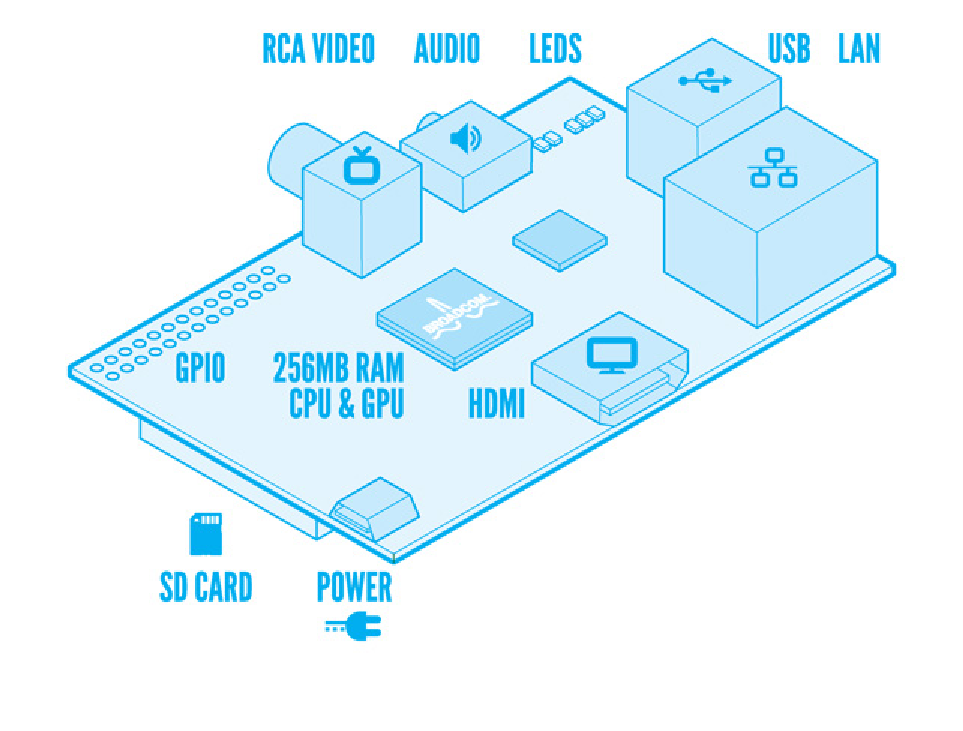
\includegraphics[keepaspectratio=true,scale=0.5]{figuras/referencialteorico/raspberry.eps}
	\caption{Raspberry Pi Model B+}
	\label{rasp}
\end{figure}

Ainda será utilizada uma tecnologia de conexão remota chamada SSH, que consistem em "um programa utilizado para acessar remotamente máquinas e executar comandos remotamente na máquina acessada" (BSD General Commands Manual, acessado em 22 de Outubro de 2015).

\subsubsection{Python}

Uma das linguagens a ser adotada será Python devido a facilidade de existir bibliotecas específicas que controlam o GPIO (\textit{General Purpose Input/Output}) do Raspberry Pi. Essa linguagem é uma linguagem de programação de alto nivel, interpretada, orientada à objetos, de tipagem dinâmica. Tem uma sintaxe consisa e clara, juntamente com uma biblioteca com recursos poderosos. Os módulos e \textit{frameworks} ainda não foram decididos.

\subsubsection{Ambiente de desenvolvimento}

O ambiente utilizado para desenvolver o \textit{software} relativo ao projeto tem como linguagem de desenvolvimento Python 3.4 e ambiente para testes.

Os testes unitários são utilizados de forma a testar a menor unidade do \textit{software}, de tal forma a suportar a automatização dos mesmos, de forma independente entre os testes \cite{unittest}. O \textit{framework} a ser utilizado será o "unittest", suportado e provido pelo próprio Python.

Ainda será utilizado o \textit{Mock}, uma biblioteca de teste que faz parte do \textit{framework} "unittest". É utilizada para simular o comportamento de um componente enquanto este não for implementado \cite{unittest_mock}.

Será realizada ainda a cobertura de código, uma métrica quantitativa de qualidade utilizada para aferir a quantidade percentual de teste do \textit{software}, mostrando assim a efetividade dos testes realizados, artifício esse que se torna indispensável quando utiliza-se testes unitários, pois proporciona um retorno da medida da eficácia.

\subsubsection{Arquitetura}

"É um conjunto de elementos arquiteturais (de dados, de processamento, de conexão) que possuem alguma organização. Os elementos e sua organização são definidos por decisões tomadas para satisfazer objetivos e restrições" \cite{arquitetura_definition}.

\subsubsection{Controle do motor}

Geralmente motores precisam de corrente relativamente altas para controlar o seu funcionamento, assim é necessário que o sistema seja capaz de drenar corrente suficiente para os dispositivos. Considerando a característica dos motores de corrente contínua, sua direção é controlada pelo sentido da corrente, pode-se construir um sistema para o controle do sentido de forma simples utilizando apenas chaves, transistores e o circuito de ponte H.

\textbf{Ponte H}

Para realizar o controle dos motores elétricos de corrente contínua é necessário determinar o sentido da corrente que passa pelos terminais do motor, é através da ponte H que se realiza o controle. Com a ponte H é possível determinar o sentido que o eixo girará e sua velocidade. O Diagrama da ponte H pode ser visto na figura \ref{fig:ponteh}.

\begin{figure}[!htb]
	\centering
	\includegraphics[keepaspectratio=true,scale=0.5]{figuras/referencialteorico/figurax.eps}
	\caption{Ponte H completa e circuitos de acionamento}
	\label{fig:ponteh}
\end{figure}

A ponte H é utilizada para o controle dos motores e ela faz isso por meio do controle de corrente. E ainda é usada para determinar o sentido de corrente e o valor de tensão no controle de um motor DC.

A ponte H é um conjunto de quatro transistores, ligados de formas que suas entradas, ao serem acionadas, polarizem apenas dois transistores como mostrado na figura \ref{fig:ponteh_fets}, dos quatro presentes. Permitindo assim, que a corrente flua pelo motor movimentando-o.

\begin{figure}[!htb]
	\centering
	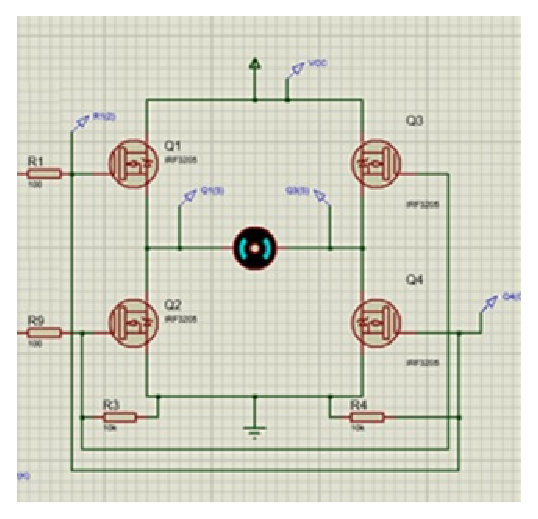
\includegraphics[keepaspectratio=true,scale=1]{figuras/referencialteorico/figurax_1.eps}
	\caption{Ponte H com transistores FETs}
	\label{fig:ponteh_fets}
\end{figure}

Os transistores da ponte H funcionam como chaves controladas por tensão. Os transistores utilizados são o IRF 3205, e eles são polarizados quando se cria uma diferença de tensão entre o \textit{Gate} (G) e \textit{Source} (s), conforme pode ser visto na figura \ref{fig:portas_transistor_irf}, VGS maior que a tensão de threshold (VTH).

\begin{figure}[!htb]
	\centering
	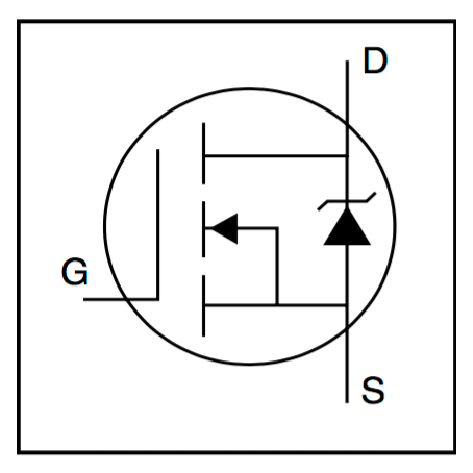
\includegraphics[keepaspectratio=true,scale=0.8]{figuras/referencialteorico/portas_irf_3205}
	\caption{Portas do transistor IRF 3205 \cite{datasheet_irf_3205}}
	\label{fig:portas_transistor_irf}
\end{figure}

A tensão de VTH é a menor diferença de tensão que precisa ser alcançado entre G e S, conforme pode ser visto na figura x, para que o transistor seja ativado essa informação encontra-se no datasheet, para o transistor IRF 3205 esse valor vai de 2V até 4V \cite{datasheet_irf_3205}.

Com isso utiliza-se desta propriedade e da disposição deles para fazer o controle do sentido de giro do motor. Quando o transistor Q1 e Q4 são polarizados, o terminal direito do motor fica com uma tensão mais positiva que o esquerdo, fazendo a corrente fluir da direita para a esquerda como mostrado na figura \ref{fig:motor_clockwise}.

\begin{figure}[!htb]
	\centering
	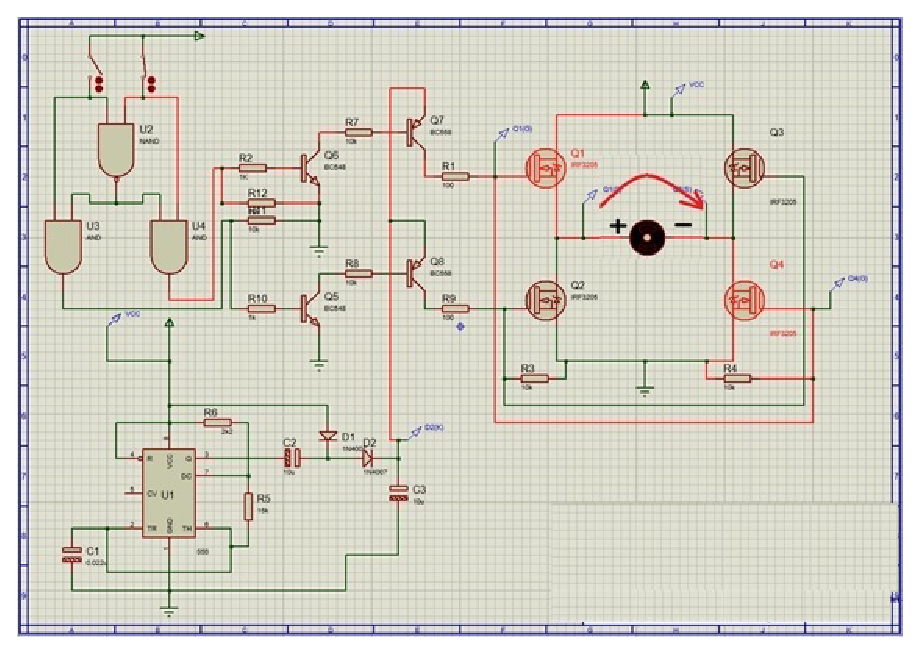
\includegraphics[keepaspectratio=true,scale=0.5]{figuras/referencialteorico/figurax_2.eps}
	\caption{Motor no sentido horário devido a corrente}
	\label{fig:motor_clockwise}
\end{figure}

Acionando-se em conjunto os transistores Q3 e Q2, o terminal esquerdo do motor fica com uma tensão maior que o direito, fazendo a corrente fluir da esquerda para a direita. Com o acionamento dos transistores Q1 e Q4, como mostrado na figura \ref{fig:motor_counterclockwise}, a corrente flui no sentido contrário e os motores giram no sentido contrário.

\begin{figure}[!htb]
	\centering
	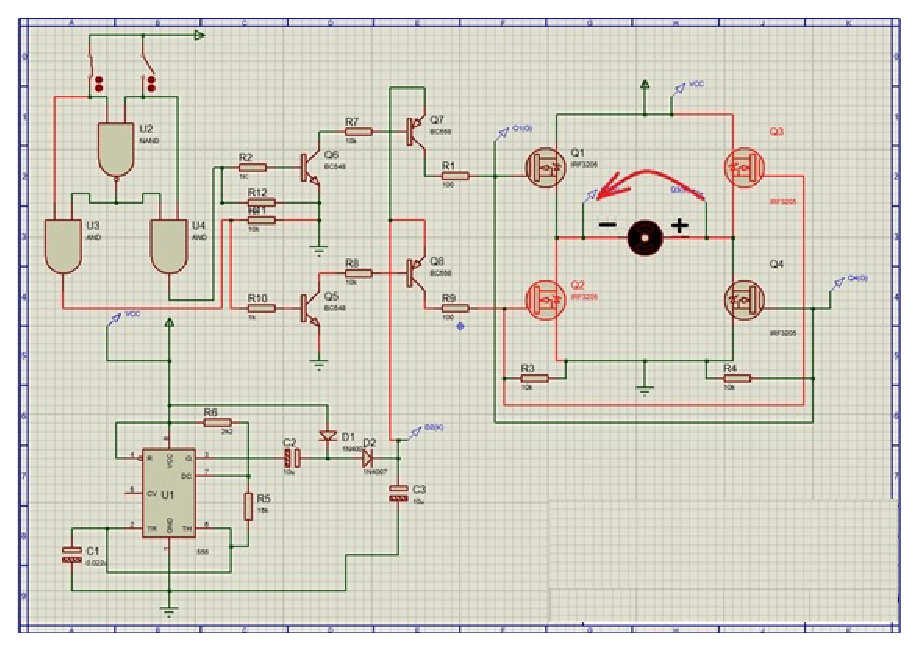
\includegraphics[width = 0.75\textwidth]{figuras/referencialteorico/figurax_3.eps}
	\caption{Motor no sentido anti-horário devido a corrente}
	\label{fig:motor_counterclockwise}
\end{figure}

Os transistores Q1 e Q2 não podem ser polarizados simultaneamente assim como os transistores Q3 e Q4. Pois o fechamento em conjunto de tais chaves causaria um curto na fonte de alimentação. Por esse motivo foi desenvolvido um modulo de segurança utilizando portas logicas na entrada, impedindo que as duas entradas que controlam os transistores sejam acionadas ao mesmo tempo.
